
\subsubsection{Interface}
\label{sec:Interface}

The \sbol{Interface} class (shown in \ref{uml:interface}) is a way of explicitly specifying the interface of a \sbol{Component}. 

\begin{figure}[ht]
\begin{center}
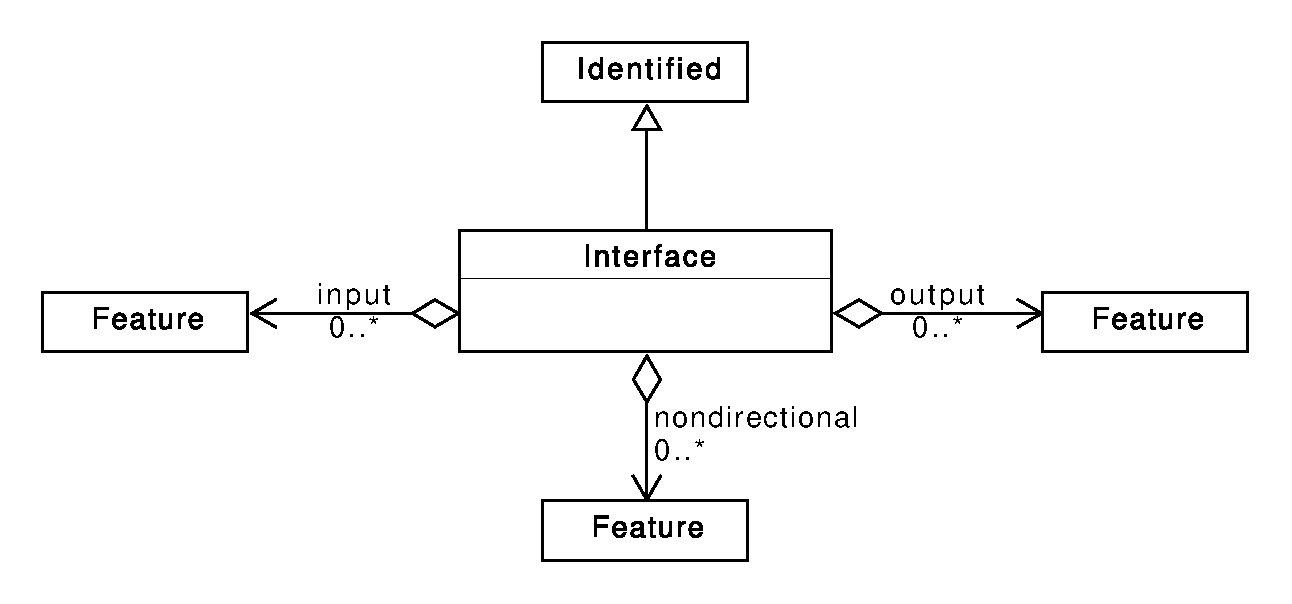
\includegraphics[scale=0.6]{uml/interface}
\caption[]{Diagram of the \sbol{Interface} class and its associated properties.}
\label{uml:interface}
\end{center}
\end{figure}

\subparagraph{The \sbolheading{input} property}
\label{sec:input}

An \sbol{Interface} MAY have any number of \sbol{input} properties, each of type \sbol{URI}, that MUST reference a \sbol{Feature} object in the same \sbol{Component}.

\subparagraph{The \sbolheading{output} property}
\label{sec:output}

An \sbol{Interface} MAY have any number of \sbol{output} properties, each of type \sbol{URI}, that MUST reference a \sbol{Feature} object in the same \sbol{Component}.

\subparagraph{The \sbolheading{nondirectional} property}
\label{sec:nondirectional}

An \sbol{Interface} MAY have any number of \sbol{nondirectional} properties, each of type \sbol{URI}, that MUST reference a \sbol{Feature} object in the same \sbol{Component}. Note that nondirectional can imply both bidirectional as well as situations where there are no flows (for instance -- a physical interface).
